\documentclass[12pt]{article} 
\usepackage{amsmath} 
\usepackage[dvips]{graphicx}
\usepackage{multirow} 
\usepackage{geometry} 
\usepackage{pdflscape}
\usepackage[labelfont=bf]{caption} 
\usepackage{setspace}
\usepackage[running]{lineno} 
% \usepackage[numbers,sort]{natbib}
\usepackage[round]{natbib} 
\usepackage{array}
\usepackage[table]{xcolor}
\usepackage{xr}

\newcommand{\methods}{\textit{Materials \& Methods}}
\newcommand{\SI}{\textit{Appendix}~}

\topmargin -1.5cm % 0.0cm 
\oddsidemargin 0.0cm % 0.2cm 
\textwidth 6.5in
\textheight 9.0in % 21cm
\footskip 1.0cm % 1.0cm

\usepackage{authblk}

\title{Do motif roles provide unique information about species risk of extinction?}

\author{Anna \r{A}kesson$^{1\dagger}$, Alyssa R. Cirtwill$^{3}$, Kate Wootton$^{2}$, Gyuri Barab\'{a}s$^{1}$, Anna Ekl\"{o}f$^{1}$} 
\date{\small$^1$Department of Theoretical Biology, Chemistry, and Physics\\ 
Link\"{o}ping University\\
Link\"{o}ping, Sweden\\
\medskip
\small$^2$ Swedish Agricultural University\\
Uppsala, Sweden\\
\medskip
\small$^3$Department of Agricultural Sciences\\
University of Helsinki\\
Helsinki, Finland\\
\medskip
$^\dagger$ Corresponding author:\\
}


\begin{document} 
\maketitle 
\raggedright

\setlength{\parindent}{15pt} 
\begin{spacing}{2.0}

% Maybe Proc B - approached Alyssa re: other motifs paper, flexible length limit.

\section*{Abstract}

    % In the Bayesian network framework, only the stable motifs are included.
    % We show that even in this case participation in different motifs is associated with different extinction risk.
    % Participation in different motifs is also correlated with in-degree and trophic level.
    % In a Bayesian network, trophic level has a very large effect on extinction risk, and likely explains a lot of what we observe for degree.
    % However, the trends we observe for motifs are not totally explained by the correlations of motifs with trophic level and degree, indicating that both simple and meso-scale descriptions of species roles provide unique information about extinction risk.

    % Omnivory may be stabilizing at high connectances because there is a low-TL "rescue prey" available to a high-risk, high-TL species. At lower connectances, perhaps higher-TL species encounter fewer disturbances and the rescue prey is less important?
    % In Lotka-Volterra systems, where top-down effects can also cause extinction, omnivory tends to be associated with less persistence. This suggests that what happens in real systems could depend on the dominant type of regulation. 
    

    % - Add a panel showing in-degree at different TL's, like in Anna's fig. Or switch to persistence vs. in-deg for each TL in a panel.
\clearpage
\section*{Introduction}

    %\subsection*{1 Why are bottom-up effects important for understanding stability?}
     The plant community is the foundation upon which the myriad of species in food webs depend for their survival \citep{}. Disturbances in the plant community have been shown to affect important ecosystem properties such as primary \citep{} and secondary production \citep{}, soil respiration and carbon cycling \citep{} and consumer diversity \citep{scherber2010bottom, Baiser2016}. The stability of the plant community is crucial for sustaining a healthy energy flow in the ecosystem as a whole \citep{Rosenblatt2016} and the structure of the plant community promotes stability across all different levels of ecosystem organization \citep{proulx2010diversity,scherber2010bottom}. Loss of diversity at the basal level typically causes declines in both abundance and richness of all types of consumers, e.g. herbivores, predators, and parasitoids \citep{scherber2010bottom}.
     %This has been shown in both theoretical work~\citep{} and empirical experiments ~\citep{} and results from the vertical propagation of disturbances through the network of interacting species.
    
     %\subsection*{2 Bayesian networks are a fantastic way to model bottom-up effects}
    The study of how an initial population decline or extinction leads to loss of other species via direct and indirect effects (i.e., secondary extinctions) is a vibrant area of research \citep{curtsdotter2011robustness, dunne2009cascading, Eklof2006}. Traditionally, there are two main approaches for studying secondary extinctions. First, there are topological models, which are solely based on food web structure \citep{dunne2009cascading}. Here, initial extinctions only affect other species in the network once a consumer has lost all of its prey and therefore must go extinct. The second approach uses dynamical models, which explicitly simulate population dynamics using a system of differential equations \citep{binzer2011susceptibility}. Dynamical models take changes in prey or predator densities into account when calculating the densities of other species in the network. These models therefore describe complex effects such as indirect interactions and are generally more realistic than topological models. However, dynamical models are parameter intensive, can only include a limited number of species, and simulations are time-consuming. 
    
    
    A middle‐ground approach for simulating secondary extinctions are Bayesian networks \citep{Eklof2013}. In this framework, a consumer's probability of extinction depends on the fraction of resources lost and on a baseline probability of extinction which captures causes unrelated to the network structure (e.g., disease, stochastic extinction of small populations). Modelling Bayesian networks is fast and computationally efficient, allowing analysis of networks with high species richness \citep{Haussler2020}. 
    As consumers do not affect the extinction probabilities of their resources, Bayesian networks can only capture bottom-up effects of disturbances within networks. However, Bayesian networks do capture the majority of secondary extinctions captured by dynamical models \citep{Eklof2013}.
    This emphasizes the importance of bottom-up effects in food webs and makes Bayesian networks the ideal framework to use when studying them.  

    %\subsection*{3 Global scale network properties are known to affect stability}
    The global structural properties of ecological networks have implications for their functioning \citep{Petchey2002}, stability \citep{Allesina2012} and robustness to disturbances \citep{Dunne2002d, Eklof2006}. For example, more highly connected networks are more resistant to secondary extinctions \citep{Dunne2002d, Eklof2006} and a modular organization, where some groups of species are tightly interconnected with limited connections between groups, can limit the propagation of disturbances \citep{}.
    %\subsection*{4 meso-scale nw propoerties also affect stability}
    Structural properties on the local scale, i.e. properties of single species, are also well-studied and there is consensus that species with high trophic levels, few prey (low in-degree), and low abundances are generally at higher risks of secondary extinction \citep{binzer2011susceptibility}. However, in-degree and trophic level are both relatively coarse descriptions of a species' role within its food-web~\citep{Cirtwill2018FoodWebs}. 
    For example, specialists may not necessarily have a high risk of extinction if it consumes a basal resource which is at low risk of being affected of disturbance. On the other hand, a consumer with low trophic level may still be at high risk of extinction if it consumes preys which possess high risk of being affected by disturbance. 
    
    
    %\subsection*{5 Motif participation may similarly affect species' particular extinction risk}
    One way to incorporate more nuance into descriptions of how species fit into their communities is to define species' roles based on their participation in different motifs -- unique combinations of small numbers of interacting species~\citep{Stouffer2007,Stouffer2012}. Importantly, these motif roles capture information about species' direct and indirect interactions, incorporating larger-scale network structure into species-level descriptions. 
    This means that two species with the same in-degrees and trophic levels can still have quite different motif roles if, for example, one interacts with specialists and the other interacts with generalists~\citep{Cirtwill2018FoodWebs}. This extended description of species structural roles may give additional information of extinction risk. 
    At the network level, the frequencies of different motifs is associated with community stability \citep{prill2005dynamic, bascompte2005simple}.
    Some motifs, such as the three-species chain, are likely to retain all species within them when modelled in isolation~\citep{Borrelli2015a} and over-represented in empirical food webs~\citep{Stouffer2007}.
    This suggests that some motifs may increase network stability by reducing the probability that species participating in them will go extinct.
    The plant community has been shown to be particularly relevant for how the motifs are distributed within a network. For example, a recent study in experimental grasslands showed that changes in the plant community, i.e. richness, induced shifts in the relative frequency of motifs in the food webs studied \cite{giling2019plant}. 
    
    %\subsection{6. only 4 (stable) motifs can appear in Bayesian networks, so how do we expect them to affect stability in a bottom-up context?}
    Of the 13 three-species motifs that can occur in empirical food webs there are four motifs that are over-represented in empirical networks \citep{Stouffer2007} and contribute to stability \citep{Stouffer2007, Borrelli2015a, giling2019plant}: the three-species chain, omnivory, apparent competition and direct competition motifs.
    These four motifs are also the only ones which can occur in the acyclic networks required for Bayesian network simulations~\citep{Eklof2013}. Because of this restriction, we only consider these four particularly important motifs.  
    

       %\subsection*{Here we test...}
    Here we are interested in how disturbances at the basal level in food webs propagate up the network and whether a consumer's extinction risk depends on 1) the motif profile of the full food web and 2) the motifs in which a focal species participates. In particular, we want to understand whether the information provided by motifs can be explained by the classical global and local food web properties such as network connectance and species trophic level, or whether motifs provide unique insight into bottom-up extinction cascades.
  
    
   % \subsection*{Other, simpler measures of species' roles can also affect extinction risk, and may correlate with motif participation}

    	%Species with high trophic levels may be more likely to go extinct since they depend upon the stability of relatively long food chains~\citep{}. 
        %For the same reasons, the number of motifs a species participates in will also tend to be larger in larger and more-connected networks.
    	%Likewise, the range of possible trophic levels increases with network size, although higher connectance may keep trophic levels low as long as the shortest food chain carries more weight (as in prey-averaged and shortest path trophic levels). 
        %A species' trophic level in turn may affects a species' motif role by restricting the set of positions in which it can appear~\cite{Cirtwill2018EcolLett}. 
    	%To unravel to what extent species motif roles gives additional information on species' probabilities of going extinct, we therefore need to take network structure and other role definitions into account.

    	
\section*{Methods}

	\subsection*{Initial network construction}

		We generated a realistic set of simulated networks based on the niche model~\citep{Williams2000,Stouffer2007} using the function "nichemodel" within the Julia~\citep{Julia} package \emph{BioEnergeticFoodWebs}~\citep{bioenergfw,Delmas2017}. 
		To capture a range of plausible network architectures, we simulated networks with sizes ranging from 50 to 100 species (in steps of 10) and connectances ranging from 0.02 to 0.18 (in steps of 0.04). 
		For full details, see~\citet{Cirtwill2021_inprep}.
        We then filtered these simulated networks to remove any with unreasonable structures.
		Specifically, we removed any network containing disconnected components (species or groups of species not connected to the rest of the network) or any network where the shortest path between a consumer and the closest basal resource was \textgreater6 (as these high trophic levels are very uncommon in empirical food webs ~\citep{}).
		New networks were simulated to replace any removed networks, and this process was repeated until we obtained 100 suitable networks in each combination of size and connectance.
              
		A Bayesian food web depicts probabilistic relationships among a set of species where each species' probability of persistence depends upon the probabilities of its resource species persisting~\citep{Jensen_Nielsen,Eklof2013}. 
		Therefore, all persistence calculations follow a strict bottom-up routine beginning by determining the status of the primary producers (who do not depend on other species) and continuing on to primary consumers (who depend only on primary producers), and so on up the network.
		
		While the niche-model food webs can contain cycles (e.g., species A eats B, B eats C, and C eats A), such cycles make it impossible to calculate persistence in the Bayesian network framework~\citep{Tarjan1972}. We therefore removed any cycles within each network.
		To render networks acyclic, we followed~\citet{Allesina2009} and broke cycles by removing links which do not contribute to the robustness of the food web.
		This is achieved by first finding the set of resources for each consumer and then removing the consumer-resource connections which have the lowest eigenvalue centrality~\citep{Allesina2009}.
		These links have the least effect on the overall stability of the network; removing them creates an acyclic network with very similar properties to the original network.
		Next, we order the species from lowest to highest trophic level using a topological sorting routine following \citep{Tarjan1972, Allesinaetal2005}, ensuring that probability calculations follow a strict bottom-up order. 
        After these steps, calculations of persistence probabilities can begin.

	\subsection*{Calculating persistence}	

		First, we assigned all species a baseline probability of extinction ($\pi_{base}$) -- the risk of going extinct given factors not related to the food web itself. 
		For consumer species, this also applies to extinction despite all resources being present. 
		Such events can, for example, reflect diseases or stochastic extinctions of small populations. 


		As well as this baseline scenario, we simulate a set of scenarios where primary producers get a higher baseline probability of extinction ($\pi_{disturbed}$). 
		These scenarios reflect threats to primary producers such as increased temperatures resulting in droughts, making some species more vulnerable to extinction.
		$\pi_{disturbed}$ ranged between $0.1-0.5$, in steps of $0.08$. The highest disturbance level, $\pi_{disturbed} = 0.5$, corresponds to basal species having a 50\% risk of going extinct. 
		Consumer species retained $\pi_{base}=0.1$ in all cases.
		
		
		As well as the intrinsic baseline probability of extinction, extinction risk for consumers is affected by access to resources. 
		When all resources are extant, the probability of extinction for a consumer $i$, $P(\lnot i)$, is equal to the baseline probability; $P(\lnot i|X_{1},...,X_{n}) = \pi_{base}$. 
		When all resources are extinct, the consumer will go extinct; $P(\lnot i|\lnot X_{1},...,\lnot X_{n})=1$. 

		Calculating $P(i)$ or $P(\lnot i)$ is less straightforward when a consumer $i$ loses a fraction $k/n = f$ of its prey. 
		Plausible ecological responses to losing some prey include i) a topological response, where the consumer's probability of extinction is constant unless all resources are lost, ii) a linear response, in which the extinction probability increases linearly with resources loss, and iii) several nonlinear responses where the probability of extinction increases non-linearly with the fraction resource lost. 
		The extinction probability will differ depending on the response function. 
		We use a sigmoid non-linear functional response of consumers to the loss of resources ($\alpha >1, \beta >1$) which has been shown to most accurately capture the secondary extinctions produced by a dynamical model~\citep{Eklof2013}. 
		We use a cumulative density function of a beta distribution for this purpose:
		\begin{equation}
		\label{betafunc}
		P(\lnot i|f) = \pi_{i} + (1 - \pi_{i}) \frac{B(f;\alpha,\beta)}{B(\alpha,\beta)}
		\end{equation}

		We calculate the fraction of resources lost ($f$) for each consumer $i$, to compute $P(\lnot i|f)$. 
		Persistence is determined by comparing $P(\lnot i|f)$ with a randomly drawn number from a uniform distribution between 0-1. 
		If this random number is lower than $P(\lnot i|f)$, the species is considered extinct. 
		The species' marginal probability of persistence is simply $P(i) = 1-P(\lnot i)$.
		In this manner we calculate persistence probabilities for all species in the network, starting from the bottom and working our way up. 
		Probabilities of extinction for resource species are used when calculating probabilities for higher level species. 
		Some species will be extinct due to primary extinctions (stochastic extinction with all resources left), while others will experience secondary extinctions; as a response to primary extinctions (partial or total loss of resources). 
		As this method is probabilistic, repeating the simulation will yield different results. 
		To minimize the effect of this variation we repeat these calculations 100 000 times per web, with unique random draws when calculating $P(i)$.
		The final persistence for each species is the mean over these runs. 

	\subsection*{Defining motif profiles and species roles}

        As a first measure of the meso-scale structure, we calculated the `motif profile' of each network.
        This is, in our case, a four-dimensional vector of the number of each three-species motif in the network.
        To separate differences in motif structure from differences in network size, we normalized motif profiles by dividing the count of each motif by the total count of all motifs.
        The motif profile for each network therefore describes the proportions of each motif and has a sum of excatly one.

    
        We then describe meso-scale structure at the species level by defining each species' motif participation and species' roles.
        Motif participation describes the frequency with which a focal species appears in each of the four motifs, analogous to the network motif profile~\citep{Stouffer2012}.
        A species' role describes the frequency with which a focal species appears in each \emph{unique position} (e.g., top, middle, or bottom species in the three-species chain, top or bottom species in the apparent competition motif) within each motif ~\citep{Stouffer2012,Cirtwill2017}.
		We calculated species' motif participation and roles using the Python package \emph{pymfinder}~\citep{pymfinder}.
        As with motif profiles of networks, we normalized participation (and role) vectors by dividing each count by the total number of motifs (motif positions) the species appears in.
        Note, however, that this normalization does \emph{not} control for differences due to degree \emph{per se} as high-degree species also tend to participate in different types of motifs than low-degree species~\citep{Cirtwill2021_inprep}.
        
        
        Finally, we calculated simpler measures of a species' role within its community: degree and trophic level.
		As the Bayesian network approach only accounts  bottom-up effects, out-degree (number of predators) is irrelevant to extinction risk.
		We therefore focused on species' in-degrees (number of prey).
		Note, however, that out-degree may also be important in topological simulations which include both top-down and bottom-up effects. 


		There are many definitions of trophic level available, most of which tend to be very similar~\citep{Carscallen2012}.
		Here we use shortest trophic level (STL): the length of the shortest food chain between the focal species and any basal resource~\citep{Williams2004}. 
		Basal resources have an STL of one, any species consuming a basal resource has an STL of two, etc.
        STL is therefore a measure of the minimum number of steps away a species is from any disturbance to the base of a food web.


	\subsection*{Statistical analysis} 

        \subsubsection*{How does mean persistence vary depending on network properties?}
        
            Both species richness (S) and connectance (C) are known to influence persistence in both simulation studies and empirical food webs.
            In addition, increasing the probability of extinction for basal species ($\pi_{disturbed}$ above) is intended to decrease persistence of species at higher trophic levels.
            Although these effects are not the main focus of our manuscript, we must establish these background effects before measuring the effects of meso-scale structure on persistence.
            The persistence of basal species in our simulations is determined only by their baseline probability, being either $\pi_{base} = 0.1$ or higher, dependent on $\pi_{disturbed}$.
            We therefore considered only non-basal species (i.e., those with at least one prey) throughout this manuscript.

            To test for effects of global network properties, we fit a linear regression relating consumer species' probabilities of persistence to network size, connectance, the level of disturbance to basal resources, and all interactions between them. 
            All predictors were centered and scaled before fitting the model. 
            As the three-way interaction was significant, we did not simplify the model.
            All models were fit using the R~\citep{R} base function `lm'.

        
        \subsubsection*{How do network motif profiles vary with global structure?}
        
            As well as affecting persistence directly, global network structure (i.e., size and connectance) may affect the meso-scale structure of the network.
            This is especially likely since we include only networks which can retain all initial species after 1000 rounds of simulated Lotka-Volterra population dynamics~\citep{Cirtwill2021_inprep}:  some meso-scale structures might be more likely to allow all species to persist than others in networks with different size and connectance constraints.
            We test whether networks with the the same size and connectance have more similar motif profiles using a PERMANOVA~\citep{Anderson2001} of Bray-Curtis dissimilarity among motif profiles against network size, connectance, and their interaction.
            Significance was calculated based on 9999 permutations.
            PERMANOVA tests may give false positive results if variability is not homogeneous among groups (i.e., levels of network size or connectance).
            To test whether this applies in our case, we fit an ANOVA of the dispersion of motif profiles about the centroid for each combination of network size and connectance. 
            We fit the PERMANOVA using the function `adonis', calculated dispersion using the function `betadisper', and fit the ANOVA using the function `anova', all from the R~\citep{R} package \emph{vegan}~\citep{vegan}.
            To gain a more detailed picture of how the proportion of each motif may vary with global network structure, we also fit four regressions (one per motif) relating the proportion of a motif to network size, connectance, and their interaction.
            We fit each regression using the R~\citep{R} base function `lm'.
            
        
        \subsubsection*{How does the persistence vary with motif frequency in the web?}

            To test whether networks with similar motif profiles tend to have similar mean persistences among consumers, we fit a PERMANOVA relating Bray-Curtis dissimilarity in motif profiles to the mean persistence of all consumers in a network (averaged across all levels of disturbance to basal resources).
            In case high or low mean persistences are associated with more variable network structure, we calculated dispersion of motif structure for each level of mean persistence (rounded to three decimal places to allow multiple networks to have the same value of mean consumer persistence and treated as a categorical variable). 
            We then tested whether dispersion was homogeneous across levels of persistence using an ANOVA and whether there was a linear relationship between persistence (rounded to three decimal places) and variability of motif profiles using a linear regression.
            All statistical tests were conducted as described above.
            
            
            To supplement these overall tests, we also fit four regressions testing whether persistence had a linear relationship to the proportion of a network profile made up of each motif, and whether this varied with the level of disturbance.
            Each regression included the proportion of a motif, disturbance, and their interaction as predictors.
            All regressions were fit using the R~\citep{R} base function `lm'.
        
        
        \subsubsection*{How does species persistence vary with motif participation?}

            We are interested in whether having a greater proportion of a species' role be made up of a certain motif (e.g., direct competition) might increase persistence.
            % (see \emph{Appendix SXX} for relationships between persistence and counts of motifs).
            To test this, we fit four linear mixed-effect models (LMMs; one per motif included in the Bayesian networks).
            These models included the proportion of the species' role made up by the focal motif, the level of disturbance to basal species, and the interaction between the two.
            We centered and scaled the predictors before fitting the LMMs.
            The models also included a random intercept for the interaction between species richness and connectance (equations.
            All models were fit using the R~\citep{R} function `lmer' from the package \emph{lmerTest}~\citep{lmerTest}.
            We calculated marginal (fixed effects only) and conditional (fixed and random effects) $R^2$ using the R~\citep{R} function `r.squaredGLMM' from the package \emph{MuMIn}~\citep{MuMIn}.

            The formula for these LMMs are:       
            
            \begin{equation}
                \Psi_{ik} \approx \rho_{i} + \pi_{disturbed_k} + \rho_{i}\pi_{disturbed_k} +
                S:C_{i} ,
                \label{propreq}
            \end{equation}


            where $\Psi_{ik}$ is the persistence of species $i$ during disturbance level $k$, $\rho_{i}$ is the proportion of the role of species $i$ that is made up by the focal motif, $\pi_{disturbed_k}$ is the probability of extinction for a basal resource in disturbance level $k$, and $S:C_{i}$ is a random intercept for the species richness and connectance of the network containing species $i$.
    
            We were also interested in whether these general trends were consistent across networks with different global properties and different levels of disturbance. 
            To test this, we performed a linear regression of persistence against motif participation within each simulated network, for each level of disturbance to basal resources.
            These regressions were fit using the R~\citep{R} base function `lm'.
            We then analyse the distribution of slopes for the effect of motif participation across levels of disturbance, network size, and connectance. 
        

        \subsubsection*{How does persistence vary with degree and trophic level?}
        
            Species' motif roles are often related to their degrees and trophic levels.
            To understand how this may have affected the results above, we first fit two linear mixed effects regressions relating persistence to degree or trophic level, $basal_p$, and their interaction.
            As above, we centered and scaled the predictors.
            We also included a random effect of the interaction between network size and connectance in order to account for the differences in persistence between different networks. 
            These regressions provide context about how persistence varies with simpler measures of species' roles within networks.
                    
        
        \subsubsection*{How does motif participation vary with degree and trophic level (i.e., do simpler measures completely explain motif results)?}

            A further complication when trying to understand whether relationships between motifs and probability of extinction depend upon underlying relationships between degree or trophic level and extinction 
            We also fit linear mixed effect models relating the proportion of each motif to degree or trophic level and a random effect of the interaction between network size and connectance using the R~\citep{R} function `lmer' from the package \emph{lmerTest}~\citep{lmerTest}.

        
        \subsubsection*{How does persistence vary with motif positions?}
        
            As one more level of detail, we can consider the frequency with which a species appears in each \emph{position} in each motif. 
            Different positions are associated with different numbers of predators and prey, making the similarities and differences between motifs and degree more explicit.
            The full set of these positions, across all motifs, is the species' \emph{motif role}~\citep{Stouffer2010,Cirtwill2017}.
            As with motif participation, we normalized motif roles by dividing the number of times a species appeared in each position by the total number of times it appeared in all positions~\citep{Baker2015,Cirtwill2017}.
            
            
            [[Could add a PERMANOVA to show that species' roles overal affect their persistence. Haven't done so yet.]]
            

            To test whether participating in different motif positions was related to a species' probability of persistence, we fit similar models to those for motif participation.
            For each position, we fit a linear mixed effect model relating persistence to the frequency of the position in a species' motif role, disturbance, and their interaction.
            To account for differences in persistence across networks of different size and connectance, we included a random effect of the interaction between size and connectance.
            All regressions were fit using the R~\citep{R} function `lmer' from the package \emph{lmerTest}~\citep{lmerTest}.


        \subsubsection*{How do motif roles vary with other network properties?}
        
            As with network motif profiles and motif participation, species' motif roles may vary with network size and connectance and with the species' in degree and trophic level.
            To identify these relationships, we fit two linear regressions for each motif position.
            The first related the frequency of the position in species' roles to network size, connectance, and their interaction.
            The second related the frequency of the position to in-degree, STL, and their interaction.
            All regressions were fit using the R~\citep{R} base function `lm'.
            
            

\section*{Results}

We are interested in i) how a the distribution of motifs in a network affect network persistence, and ii) how a species motif profile affects its persistence. We analyse this for different levels of disturbance to the basal level. 

The results are organized as follows: 1) How network persistence varies with network motif distribution. 2) How network persistence varies with global structural properties. 3) How network motif distribution varies with global structural properties. 4) How species probability of persistence varies with its motif profile. 5) How species persistence varies with its characteristics such as TL and in-degree. 6) How a species motif profile depend on its characteristics. 7) How a species persistence  varies with its motif role (position in respective motif). 
    
    \subsection*{Network persistence and level of disturbance and global network properties}
    The level of disturbance naturally had clear and profound effects on the average network persistence, such as a increased probability of extinction of basal species always decreased network persistence. 
  
    Network size and connectance affect persistence, but to a much smaller extent than increasing disturbance (Figure S1, Table S1, \emph{Appendix SA}). Persistences generally decrease when networks are more connected, but the effect of network size varies depending on level of disturbance. At low disturbance, small and highly-connected webs show the lowest persistence, whereas at high disturbance, large and highly connected webs show the lowest persistence (Fig. S2, \emph{Appendix SA}).


    \subsection*{Network motif profile and global network properties}

        Considering each motif separately, the proportions of apparent competition and three-species chains in a network's motif profile tended to decrease with increasing connectance while the proportion of omnivory increased with increasing connectance (Table S2, \emph{Appendix SB}). Network size and the interaction between network size and connectance did not strongly affect the frequencies of most motifs (Fig.~\ref{motif_proportion_lms}).

        \begin{figure}[h!]
            \centering
            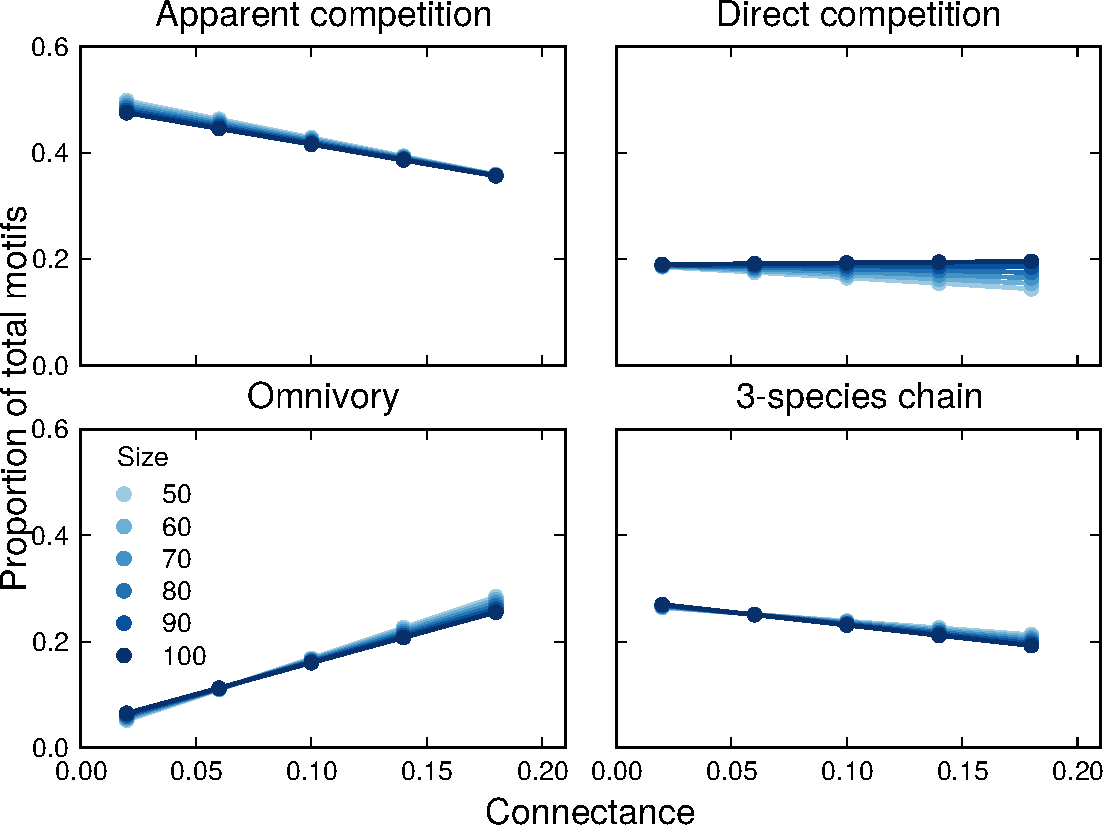
\includegraphics[width=.75\textwidth]{manuscript/figures/motif_proportion_lms.pdf}
            \caption{The proportions of a network's motif profile made up by the four motifs which can appear in acyclic networks vary with the size and connectance of the network. More-connected networks tend to contain relatively more omnivory motifs and fewer apparent competition motifs. The proportions of direct competition and three-species chain motifs were less variable.}
            \label{motif_proportion_lms}
        \end{figure}

    \clearpage

    \subsection*{Network motif profile and network persistence}
    
        The motif profile of a network is related to the average persistence of consumers ($F_{1,2998}$=571, $p$\textless0.001). Average persistence is higher in networks with higher proportions of the chain, direct competition, and apparent competition motifs (Table S3, \emph{Appendix SC}). Conversely, average persistence is lower in networks with higher proportions of the omnivory motif. These trends hold for all levels of disturbance (Fig.~\ref{motif_profile_persistence}, Table S3), \emph{Appendix SC}).% Network persistence varies between networks with different dispersion of motif profiles ($F_{134,2865}$=2.19$\times10^{24}$, $p$=\textless0.001). For example, networks with more variable motif profiles have higher persistence ($\beta$=0.183, $p$\textless0.001).

        \begin{figure}
            \centering
            \includegraphics[height=.5\textheight]{figures/persistence_motif_profiles.eps}
            \caption{The proportions of the four motifs in a network's motif profile are related to the mean persistence of species in the network. Specifically, persistence decreases as the proportion of omnivory in the network's motif profile increases while persistence increases with the proportions of the other three motifs. Interactions between motif profiles and disturbance were significant but small. Here we show the relationships of probabilities of extinction of basal resources of 0.1 (top set of lines) and 0.5 (bottom set of lines). Relationships are shown for the observed range of proportions for each motif.}      
            \label{fig:motif_profile_persistence}
        \end{figure}    


    \subsection*{Species motif participation and species persistence} 
    
       The effects of motif participation on a species persistence depend on level of disturbance. When disturbance is low species' persistence increase with increasing proportions of the omnivory and direct competition motifs. Conversely, a species' persistence decrease with increasing proportion of the apparent competition motif. Persistence is not significantly related to the proportion of the three-species chain motif (Figure~\ref{fig:prop_lmer_all}).
            
        At high levels of disturbance, species persistence decrease as the proportion of the three-species chain increase, but increase as the proportion of all other motifs increase (Figure~\ref{fig:prop_lmer_all}). This means that increased disturbance strengthened the effects of the three-species chain motif and changes direction of the effect from the apparent competition motif  (Table S4, \emph{Appendix SD}). The effect of omnivory on persistence is still positive but weaker at higher levels of disturbance, and the effect of direct competition was largely unaffected by disturbance level.
    
            
            \begin{figure}[h!]
                \centering
                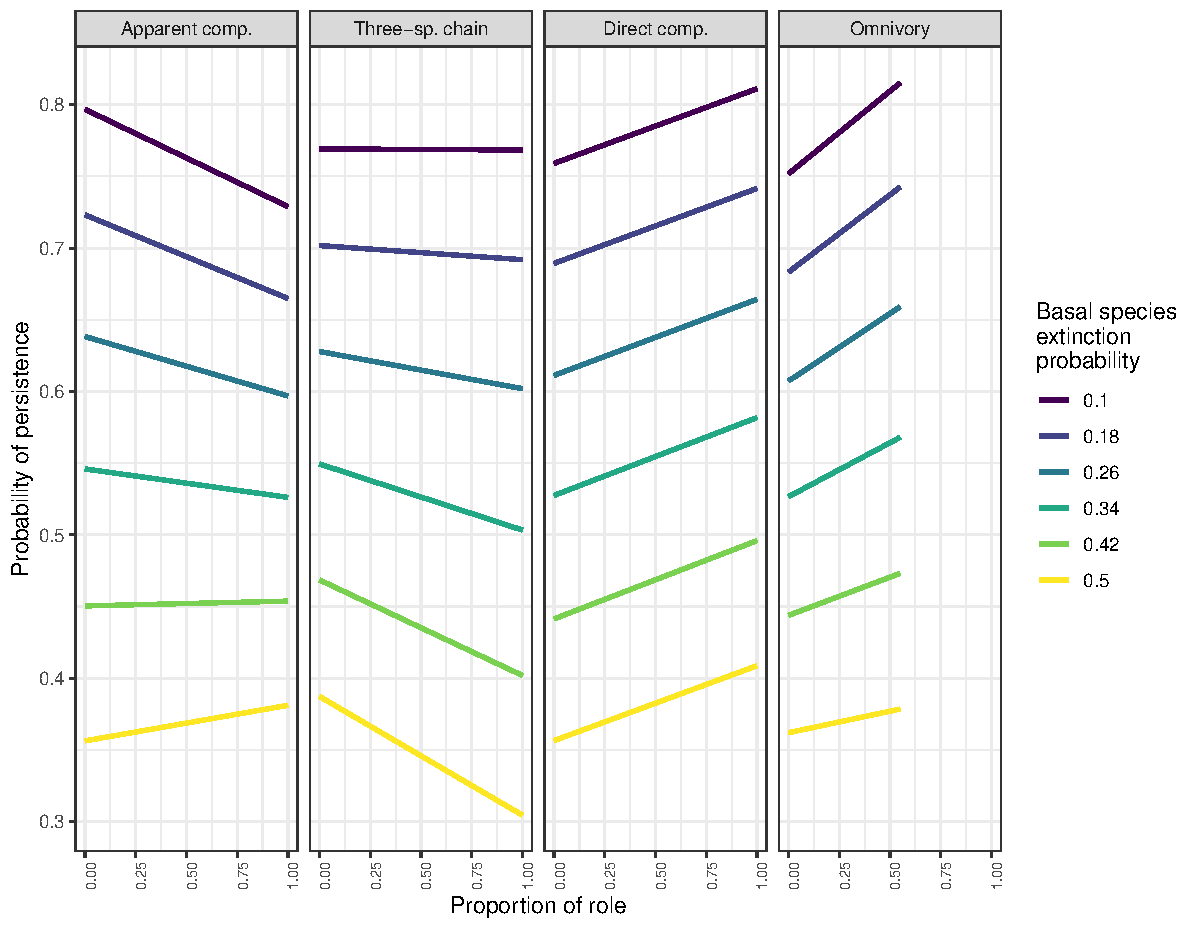
\includegraphics[width=0.85\textwidth]{figures/prop_lmer_allCS.pdf}
                \caption{The effect of proportion of the role (x-axis) made up by various motifs (columns) on persistence (y-axis). The effect of participating in each motif is based on linear mixed-effect models following Equation~\ref{propreq}, except that models for each  disturbance level are fitted separately. The different colored lines indicate the probability of extinction of basal species, from $\pi_{disturbed} = 0.1$ (top, purple; no disturbance) to $\pi_{disturbed} = 0.5$ (bottom, yellow; high disturbance). Note that omnivory made up a smaller proportion of species' roles than other motifs; lines are plotted over the observed ranges of motif participation.}
                \label{fig:prop_lmer_all}
            \end{figure}
        
        \clearpage
    
        \subsubsection*{Consistency in species persistence versus motif participation}

            In order to evaluate how consistent the relationships between a species persistence and motif participation is, and how it varies with  level of disturbance and global network structure, we fit linear regressions of species persistence against motif proportions for the species for each network separately. We then analyze the density distribution of the values of the slopes. Network size had a much smaller effect than connectance (Fig. S3; \emph{Appendix SE}); we therefore focus on connectance here. 
            
            Networks with high connectance generally have more consistent relationships between persistence and motif participation, i.e., sharper peaks of the density distributions (Fig.~\ref{fig:density_prop_C}). However, there is an interaction between disturbance and connectance for the direct competition and omnivory motifs; At low and medium connectances there is little change in the proportion of positive slopes when the proportion of  direct competition motif is high, independent of level of disturbance. At high connectances, however, the proportion of positive slopes is lower and also decreases with increasing disturbance. For the omnivory motif the trend is reversed. Additionally, the omnivory motif stands out having a wider curve when network connectance is low.


        \begin{figure}[h!]
            \centering
            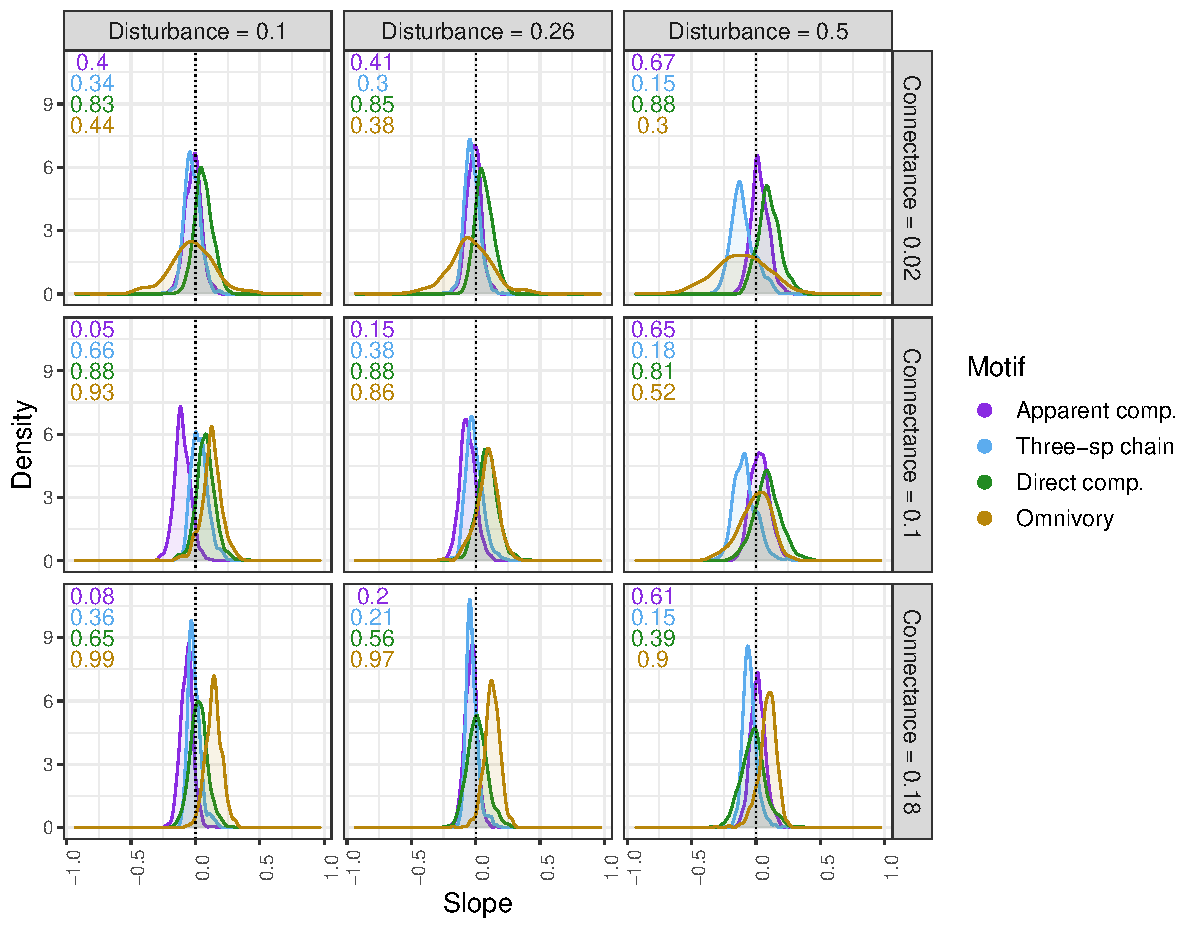
\includegraphics[width=\textwidth]{figures/prop_dens_bp_vs_C_allS.pdf}
            \caption{Density (y-axis) of slopes (x-axis) of persistence against proportion of different motifs for all simulated webs of all sizes - a visualization of how an increased proportion of each motif (different colored lines) affects persistence of consumer species. The slopes are derived from standard linear regression. Columns show the result for various disturbances on the basal level, from $\pi_{disturbed} = 0.1$ (left) to $\pi_{disturbed} = 0.5$ (right). Rows show various levels of connectance. The dotted, vertical line indicate zero on the x-axis. A negative slope value reflects a negative relationship between increased participation in a motif and persistence, while a positive slope value reflects a positive relationship - an increased proportion of a specific motif increase persistence. The fraction of replicates with a slope greater than zero are stated in numbers in each sub-plot, the color corresponding to each motif (legend). }
            \label{fig:density_prop_C}
        \end{figure}    
    
    \subsection*{Species characteristics and persistence}
    
        A species persistence varies with both species in-degree and trophic level (Fig.~\ref{fig:motifs_vs_TL_and_deg}; \emph{Appendix SF}). Increased trophic level is generally associated with decreasing species persistence, although the rate of decline is slower at high disturbance (Table S5, \emph{Appendix SF}).
        In-degree shows an even stronger interaction with disturbance, as a having more  prey species is associated with higher persistence in the no disturbance scenario, but lower persistence at high disturbance scenario.
        

        % Anna notes (just for our (mine) understanding): 
        % When looking at the two figures of degree vs persistence and STL vs persistence - my conclusion is that species at lower trophic levels have the highest in-degree. Double check - yes, that’s true.
        % Lower TL are all well at low disturbances, and when disturbance increase, persistence decrease (looking at fig degree vs persistence, right end of the line).
        % Higher TL experience the same thing, although to a slightly smaller extent (looking at the left end of the lines in fig degree vs persistence and right end of lines in fig STL vs persistence). 
        % The slope of the line in fig degree vs persistence is not really relevant, since it's kind of based on the response of different TL level (which makes perfect sense in the BN framework)
        % weird thing though - at high levels of disturbance, lower TL seems more affected than higher TL in the persistence vs degree figure (since low degree belongs to higher TL, high degree to lower TL). This does not correspond with fig persistence vs STL. HOWEVER - not only high TL have a low degree, lower TL do as well, probably affecting the overall result. Only low TL have high degree - but the opposite is not true. Probably explains it
    
    \clearpage
    
    \subsection*{Species motif participation and network properties and species characteristics}

       Species' motif roles varied depending on the properties of the network; size, connectance, and their interaction (Fig. S4, Table S6; \emph{Appendix SG}).
        Species appeared most often in the apparent competition motif in all types of networks, but the frequency decreased with increasing network size and connectance.
        The frequency with which species participated in the omnivory motif increased sharply with increasing connectance, while the frequency of the direct competition motif increased slightly with increasing network size. 
        
        Species' motif roles also varied with their in-degree and trophic level (Fig.~\ref{fig:motifs_vs_TL_and_deg}).
        Species with higher in-degree tend to have higher proportions of their motif role made up by omnivory. Proportions of the other three motifs tend to decline with increasing degree.
        Species with higher trophic levels tend to have higher proportions of apparent competition and three-species chains. 
        

            \begin{figure}
                \centering
                \includegraphics[width=\textwidth]{figures/roles_vs_TL.eps}
                \caption{As with motifs, persistence varied with simpler measures of species roles in networks. Moreover, motif frequencies correlated with in-degree and trophic level. \textbf{A-B)} Persistence increased with increasing in-degree for low levels of disturbance to basal resources but decreased with increasing degree for high levels of disturbance to basal resources.
                Persistence declined with inceasing STL for all levels of disturbance to basal resources.
                \textbf{C-D)} The proportion of omnivory increased with increasing degree while all other proportions decreased. The proportions of omnivory and direct competition decreased with increasing STL while the proportions of apparent competition and three-species chains increased.}
                \label{fig:motifs_vs_TL_and_deg}
            \end{figure}        
        

    \subsection*{Persistence and species' positioning in motifs}

        A species probability of persisting is significantly related to the frequency of all positions, disturbance, and the interaction between frequency of each position and disturbance (Table SX, \emph{Appendix SH}).
        In the omnivory motif, persistence increased with the frequency of the bottom position (two predators, no prey within the motif) across all levels of disturbance but most steeply at high levels of disturbance (Fig.~\ref{figs:persistence_position_motifs}).
        Persistence increased slightly with the frequency of the middle position (one prey, one predator) at low levels of disturbance but showed little relationship at higher levels of disturbance.
        Persistence increased with the frequency of the top position (two prey, no predators within the motif) at low disturbance but decreased at higher levels of disturbance.
        
        In the three-species chain, persistence decreased as the frequency of the top position increased at all levels of disturbance.
        Conversely, persistence increased with increasing frequency of the middle position at all levels of disturbance.
        Persistence decreased slightly with increasing frequency of the bottom position at low levels of disturbance but increased at high levels of disturbance.
        
        In the apparent competition motif, persistence decreased slightly with increasing frequencies of the bottom position (one predator, no prey within the motif) at low disturbance but increased slightly at high disturbance.
        Persistence increased with increasing frequency of the top position (two prey, no predator within the motif) at low disturbance but decreased at high disturbance.
        
        In the direct competition motif, persistence varied little with the frequency of the bottom position (two predators, no prey within the motif) at low disturbance but increased with the frequency of this position at high levels of disturbance.
        Persistence increased slightly with the frequency of the top position (one prey, no predators within the motif) at low levels of disturbance and decreased slightly at high levels of disturbance.
        

    \begin{figure}[h!]
        \includegraphics[width=.95\textwidth]{figures/persistence_positions_Omnivory.eps}
        \caption{A species' probability of persistence varied with the frequency of different motif positions in its role. Here we show the relationships between persistence and the proportions of the three positions in the omnivory motif at three levels of probability of extinction for basal resources (p=0.1, 0.26, and 0.42), indicated by line colour. Line style indicates the motif  position. }
        \label{figs:persistence_position_motifs}
        \end{figure}


        The frequencies of motif positions in a species' role varied with network properties (\emph{Appendix SI}).
        Motif roles had stronger relationships with degree and STL than with network size or connectance.
        


\clearpage

%Somewhere early in discussion (needs tidying up):
%Apparent comp and direct comp have no indirect effects in BN, so we should be able to explain them with simpler properties.
%AC is strongly negatively correlated with in-degree. Higher in degree is associated with both high persistence at low disturbance (Fig. 7A) and low participation in AC (Fig. 7C). Low participation in AC is in turn associated with high persistence at low disturbance (Fig. 4). Note that trends for degree and AC reverse at high disturbance in the same way!
%DC is not strongly correlated with degree but does decrease strongly at high trophic levels. High trophic level and low DC are both associated with low persistence at all levels of disturbance, making it likely that the effects we observe for DC are trophic level in disguise.
%Three-species chain and omnivory do have indirect effects in a BN setting, and they can't be fully explained by degree or trophic level (since the result doesn't follow the result for degree). We can see this because despite the strong correlations with degree and trophic level these motifs don't show the same patterns with persistence. We therefore focus on them here.


\section*{Discussion}
% Connect back to intro -- importance of the plant community for a healthy consumer community.
% Focus on what additional information is revealed from analyzing motif compared to global network properties or species characteristics.
% Connect to traits -- Cirtwill & Eklöf, 2018, Ecol Lett. 
% Bayesian network approach - what extra information does motifs provide when we are interested in bottom- up effects. 
% * Difference between 3-sp chain and omnivory, the importance of the rescue prey in omnivory (in dynamical sims omni was mostly bad, 3-sp chain good). Omni link destabilizing if strong, stabilizing if weak (other studies). In BN just a link as important as other links
% * Omnivory in fig 5 - high connectance, always good, not as good with lower levels of C
% * Extra prey in omnivory changes from being a security to a liability (with increasing disturbance?)
% * ADD REFS - high disturbance scenario is analogous to decreasing plant diversity


% Results summary - network level (following Anna)
Changes in the basal level in food webs have profound effects on all other species in the network \citep{}, as all consumers depend directly or indirectly on primary producers for their survival \citep{}.It has repeatedly been shown that global network properties are important for how well a network can handle disturbances, such as loss of species \citep{Eklof2006, Dunne2002}. At the same time, from a conservation perspective it is often more relevant to look at specific species to which actions can be targeted \cite{}. Nevertheless, since species do exist in a network their interactions, direct as well as indirect, will affect how they respond to a disturbance. Motifs are the basic building blocks in networks and as such represents a bridge between network-wide (global) and species-specific (local) properties. Here we were particularly interested in how the distribution of these meso-scale structures in ecological networks are related to network and species persistence when the plant community is affected by species loss.

A network's motif profile had relatively strong relationships to the network average persistence, compared to global structures, such as network size and connectance, whose effects were smaller. However, connectance (and, to a lesser extent network size) do affect network which motifs that are most prominent. Thus, global-scale properties have stronger effects on network persistence by changing meso-scale properties than directly which indicates that network motifs do provide additional information.  

% Network-level persistence
 In general, average network persistence was lowest in networks with high frequencies of the omnivory motif and highest in networks with high frequencies of the apparent competition motif. Direct competition and three-species chain motifs both showed positive but weaker relationships. The level of disturbance naturally affected the level of persistence, such as increased disturbance decreased average persistence, but trends were largely unaffected.

% About fraction of omnivory and apparent competition in the full network 
The negative relationship between omnivory and network persistence is consistent with other studies showing that an omnivory motif is less likely to be stable than the other motifs considered~\citep{Borrelli2015a}.

High frequency of the apparent competition in a network motif was correlated with an on average higher in-degree for consumers. In-degree has repeatedly been suggested to be beneficial for a species persistence  \citep{}.

Motif profiles with high apparent competition and low omnivory were also more likely in less-connected food webs, which had higher mean persistence than highly-connected food webs.
Despite these general trends, networks with more variable motif profiles had higher mean persistence, suggesting that many different network structures support high probabilities of persistence. 
High connectance might reduce mean persistence by limiting the number of possible meso-scale network structures.
In particular, it is reasonable to expect higher frequencies of the omnivory motif at high connectances since this motif contains more links than the other three-species motifs considered here.
% Top species directly connected to the disturbance, disturbance not mitigated via herbivores. Duality in the role of omnivory.
% The relationship between high connectance and frequency of omnivory motif should perhaps come earlier. 
% Close with something about how more links allow disturbance to propagate.

% Species level persistence
% What we want to discuss here: 1) Apparent competition change direction depending on disturbance. 2) High disturbance strengthen the effect of chain. 3) Omnivory most positive in low disturbance scenarios. 

While the persistence of a particular species is likely to be affected by global-scale (size and connectance) and meso-scale (motif profiles) network structure, it also depends on what characterize a species position in the network., such as trophic level, number of interactions and which motifs the species participate in.  

In our results, motif participation is significantly related to persistence, but some of the effects can to some extent be explained by local properties such as in-degree and trophic level. This is especially likely for the apparent competition and direct competition motifs, since in Bayesian Network framework lacks top-down effects and therefore the indirect effects in these motifs are not relevant. 


Participation in the apparent competition motif is strongly negatively correlated with in-degree --a high proportion of the apparent competition motif implies a low in-degree. Both higher in-degree and lower participation in the apparent competition motif are associated with greater persistence at low disturbance but decreased persistence at high disturbance. This suggests that in-degree is in fact the factor driving the positive relationship between proportion of apparent competition motif and species persistence. Interestingly though, the relationship changes from positive to negative with increasing level of disturbance. When disturbance is high having many prey species acts as an insurance, while at high disturbance connections to many prey species is in fact negative as the consumer receives the negative impact from several sources.   

However, the coupling between a species proportion of motif participation and degree is neither evident or always true. For example, it is possible for a species with low degree to participate in many motifs if it interacts with high-degree species and thereby obtain many indirect interaction partners. This is one of the strengths with analyses of motifs that it considers local structures additionally include indirect connections one link away.  


A species participation in the direct competition motif is only weakly correlated with in-degree, but is instead strongly negatively correlated with trophic level---species with a high proportion of the direct competition motif are more likely to have low trophic levels. Low trophic levels are naturally associated with higher persistence in our analyzes  as they receive less negative impact from the bottom-up disturbances ~\citep{Eklof2013}. The clear positive relationship between proportion of direct competition motifs and species persistence is therefore likely due to the tendency for species at low trophic levels to have a higher proportion of that motif. Therefore, contrary to the apparent comptition motif, we do not observe a change in the relationship with changed disturbance.

The three species chain motif have a nearly neutral relationship with persistence when disturbance is low, but a clearly negative relationship when disturbance is high. This can partly be explained with the positive relationship between trophic level and a species proportion on the chain motif. In the three species chain motif the species are on average more often dependent on two trophic levels (if the focal species possesses the top-position in the motif), and as such affected negatively from two trophic levels. A high level of disturbance (high probability for a basal species to go extinct) will then sharply decrease persistence for the top species. 

%In contrast to the two competition motifs, the three-species chain and omnivory motifs have a less evident relationship to species in-degree or trophic level. For example, the three-species chain motif is negatively correlated with in-degree and positively correlated with trophic level. Despite this correlation, participation in the three-species chain does not interact the same way with disturbance as either of the simpler measure and so has a unique relationship to species persistence. This is likely due to indirect effects of the bottom species in the chain on the top species. 


The perhaps most interesting motif is omnivory. Omnivory shows a reversed relationship with disturbance level compared to the three species chain; at low disturbance a high proportion of omnivory is positive for persistence whereas the effect is nearly neural for high levels of disturbance.    


While participation in the omnivory motif is positively correlated with in-degree, a high proportion of the omnivory motif is always associated with increased persistence, while the effect of in-degree varies with disturbance. 
Thus, the effect of a high proportion of the three-species chain motif and the omnivory motif does not follow the corresponding effect of in-degree and trophic level. 

% Two notable results: 1) omnivory bad at network level, good at species level, 2) apparent competition depends on disturbance
Combining the results from our species wise exploration with our network-level findings, we see that while being in a network with high frequencies of omnivory decreases persistence, participating in many of these omnivory motifs increases persistence at the species level.
At the network level, a higher frequency of the omnivory motif leads to more pathways by which the disturbances to basal resources can propagate and cause extinctions of consumers.
At the species level on the other hand, if extinctions of basal resources are rare, these multiple pathways will tend to protect consumers participating in many omnivory motifs by providing alternative channels of energy.
If extinctions of basal resources are common, however, these multiple pathways cause a negative impact as they will transmit more disturbances to the consumer.

Additionally, the effect of the omnivory motif on persistence was closely connected to connectance. In highly connected networks, a high proportion of the omnivory motif strongly contributed to higher persistence. This was not the case in less connected networks. 
In a highly connected network, a disturbance could potentially spread to a higher extent than in a less connected network. 
Therefore, in a highly connected web where disturbances have more ways to move, the lower level prey item in the omnivory motif may be of even higher importance assisting as a buffer, decreasing the negative effect of disturbance for the consumer species. In a less connected network, this additional prey species is of less importance.

To understand the species-level effect, we consider the relationships between stability and each position within the motif.
Appearing frequently in the top or middle positions of the omnivory motif is associated with higher probabilities of persistence at low levels of disturbance, while appearing frequently in the bottom position is associated with higher probabilities of persistence at high levels of disturbance.
This is consistent with the logic outlined for the network-level effect: when extinction of basal species is rare, consumers at the top or middle of omnivory motifs benefit from multiple energy channels but when extinction is common these multiple channels mean that the consumer is likely to be affected by multiple disturbances. The bottom position shows the reverse effect: at low levels of disturbance, this position is nearly neutral.  At high levels of disturbance, however, being low down in the motif (and obtaining energy by appearing as a predator in other motifs) means that the species is less likely to be affected by multiple lower-level extinctions.
The offsetting of effects of different positions within the omivory motif may explain why the motif as a whole is associated with greater probabilities of persistence across all levels of disturbance we considered.



% The divergent effect on persistence of either having a high proportion of the three-species chain or omnivory motif can, within our Bayesian Network framework, be explained by the structure of the food web.
% When participating in a food chain motif---three-species chain or omnivory---the top species of this structure will have a higher susceptibility since disturbances amplify through the network. In our results, this is in particular evident for the three-species chain motif at higher levels of disturbance, but this also applies to species with a high proportion of the omnivory motif. While the relationship between omnivory and persistence is strongly positive at low bottom-level disturbance, the trend is reduced at high levels of disturbance. 
% This is because species participating to a high extent in omnivory motifs share the sensitivity of species participating to a high extent in three-species chain motif, and are similarly negatively affected by bottom-level disturbances. However, the top species in an omnivory motif also have the benefit of an additional prey species, located further down in the food web. This prey item can assist as a buffer, decreasing the negative effect of disturbance on the consumer species. Clearly, this additional prey is of importance, since it is more beneficial with a higher proportion of the omnivory motif for an individual species than a high proportion of the three-species chain motif. 
% Thus, the observed benefit of a high proportion of the omnivory motif can be compared to omnivores in a network feeding adaptively. Studies have demonstrated that adaptive omnivory can increase the permanence of three-species chains \citep{Fagan1997, KrivanDiehl2005, AbramsFung2010}.
% Although species in our model cannot swap prey dependent on bottom-level disturbances or lower resource densities, a species with a high proportion of omnivory will in a sense spread its risk between prey items at different trophic levels.



% Broader context of omnivory is probably better after we introduce the species-level results. 
The relationship between omnivory and stability is subject to a longstanding debate in ecology. Omnivory has been shown to both stabilize and destabilize communities, and the impact is highly dependent on network context \citep{bascompte2005simple, MonteiroFaria2016, Kratinaetal2012}. 
For example, omnivorous interactions may not be stable in isolation, but instead stabilized by interactions with other species when embedded in a larger food web \citep{Kratinaetal2012}. Additionally, the possibility of omnivores to feed adaptively from different trophic levels can spread the risks, for example when the prey level are disturbed \citep{Fagan1997}.
This might be why we have a divergent pattern between a full food web's motif profile versus each single species motif profile.

 \cite{Cirtwill2021_inprep} analysed how species time to extinction varied depending on their network profile. They found that a high proportion of the omnivory motif resulted in a shorter time to extinction, while the other three stable motifs were associated with longer times to extinction. However, the study by Cirtwill and Wootton used a different approach using a dynamic simulation model also including top-down effects. 


    
    
    % % We can move this to the SI or delete entirely.
    % Although we performed analysis of both the effect of the absolute counts of motifs and the normalized motif role on persistence, we here focus on the normalized motif role.
    % This is because, the consistency of the relationships between persistence and the number of times a species appears in any of the possible motifs suggests that the observed effects of non-normalized motif roles are actually due to degree.
    % Species with higher degrees will with high probability appear in more motifs than species with low degrees.
    % It is possible for a species with low degree  to participate in many motifs if it interacts with high-degree species (thereby obtaining many indirect interaction partners).
    
    % When we consider the proportion of a species' role made up by each motif, the influence of degree is largely removed.
    % Given the similarly high $R^2$ values between the models using proportions of motifs and absolute counts, it does not appear that we lose much explanatory power by removing degree. 
    % Therefore, our main analysis focus on the effect of the normalized motif role on persistence.
    
[[Comparison to degree, tl?]]

    % This paragraph explains why motif trends aren't just due to TL
    Two of the focal motifs, omnivory and the three-species chain, include three trophic levels while apparent and direct competition only require two.
    However, the effects of motifs on persistence cannot be reduced to the number of trophic levels in each motif.
    The two predators in a direct competition motif or the two prey in an apparent competition motif are not necessarily at the same trophic level. This is demonstrated by the increasing participation in apparent competition and chain motifs and decreasing participation in direct competition and omnivory motifs with increasing trophic level (i.e., 2-TL and 3-TL motifs do not show consistent trends).
    In fact, a prey in a direct competition motif can have a higher trophic level than its predator.
    For example, blueberries and salmon consumed by a bear make an apparent competition motif where the salmon, a piscivorous fish, has a higher trophic level than the blueberries or the omnivorous bear.
    This means that motif participation and trophic level give complementary descriptions of a species' place in the network and explains why the simple decrease in participation with increasing trophic level does not explain the more complicated relationships between motif participation and persistence.
    
    
    In-degree (number of resources) may explain more of the relationships between motif participation and persistence.
    For example, higher proportions of the omnivory motif in a species' participation vector were associated with higher persistence for that species, and participation in omnivory significantly increased with increasing in-degree.
    Moreover, the relationship between degree and persistence  showed a strong interaction with disturbance, similar to the varying relationship between apparent competition and disturbance. 
    The shift from positive relationships between persistence and apparent competition at high levels of disturbance to negative relationships between persistence and apparent competition at low levels of disturbance could be partially explained by the negative relationship between apparent competition and in-degree.
    However, participation in the three-species chain also significantly decreased with increasing degree while participation in omnivory increased, and neither of these motifs shows a similar interaction with disturbance.
    As with trophic level, motifs provide some unique information not provided by in-degree (and vice versa). 
    Both ways of describing a species' position in the network show significant relationships to consumers' persistences after a disturbance and, because these relationships are not the same, likely capture different mechanisms leading to greater or lesser extinction risk.
    
    
 %When analyzing motifs within a Bayesian Network, it is important to keep in mind that only bottom-up effects are accounted for. Therefore, the implications of the four possible motifs are different than they would be in an empirical network.
    
    %In particular, the lack of top-down effects removes the indirect effects from the two competition motifs. In the case of direct competition, two predators share a common resource. The predators will, within a Bayesian Network, not affect each other indirectly although both will be affected by any disturbance to their resource. Similarly, the two bottom-level species in the apparent competition motif will be independent of each other as there are no top-down effects of the shared consumer to link them.
    %The difference between the direct competition and apparent competition motif is thus the number of bottom-level species, accounted for as prey items for a higher level species.
   % A predator participating in many direct competition motifs is likely to have fewer prey items than a predator participating frequently in the apparent competition motif, and therefore a higher extinction risk.Note, however, that consumers can also appear in these motifs as prey to other consumers.  In that case, we would not expect the two motifs to have different effects on extinction risk.
    %The structure of the omnivory motif and the three-species chain motif differ from the competition motifs by having an additional trophic level. Therefore, top-level species of these motifs might be more sensitive to disturbances since they can be affected by the loss of the basal resource in the focal motif or an increased probability of extinction of the middle species due to a disturbance to a basal resource not included in the focal motif.     
    
% [[When can motifs still be useful predictors and add insight?]]
%     Our results suggest that some motifs are associated with higher persistence than others but that this depends on the level of bottom-up disturbance to the food web.
%     Detailed tests of how motifs affect network stability and species persistence ideally require the ability to manipulate the motif structure of a network directly (i.e., obtaining many replicate networks with set numbers of each motif). 
%     Current methods of generating simulated ecological networks (e.g., the niche and cascade models) do not incorporate information on motifs.
%     Researchers interested in relationships between motif structure and persistence must therefore generate large numbers of networks and hope that they contain the necessary variety of motifs.
%     This shotgun approach to simulating different distributions of motifs within networks makes it difficult to investigate the precise effects of different numbers of, for example, the three-species chain motif, whether it occurs high or low in the network, and similar questions.
%     Fortunately, software is currently in development to allow researchers to simulate networks with particular motif profiles.
%     We heartily encourage researchers interested in the effects of motifs on persistence to adopt these new methods as they become available.
    


\bibliographystyle{ecollett} 
\bibliography{anna_bib_new} % Abbreviate journal titles.

\end{spacing}

\end{document}

